\documentclass[11pt]{article}

    \usepackage[breakable]{tcolorbox}
    \usepackage{parskip} % Stop auto-indenting (to mimic markdown behaviour)
    

    % Basic figure setup, for now with no caption control since it's done
    % automatically by Pandoc (which extracts ![](path) syntax from Markdown).
    \usepackage{graphicx}
    % Keep aspect ratio if custom image width or height is specified
    \setkeys{Gin}{keepaspectratio}
    % Maintain compatibility with old templates. Remove in nbconvert 6.0
    \let\Oldincludegraphics\includegraphics
    % Ensure that by default, figures have no caption (until we provide a
    % proper Figure object with a Caption API and a way to capture that
    % in the conversion process - todo).
    \usepackage{caption}
    \DeclareCaptionFormat{nocaption}{}
    \captionsetup{format=nocaption,aboveskip=0pt,belowskip=0pt}

    \usepackage{float}
    \floatplacement{figure}{H} % forces figures to be placed at the correct location
    \usepackage{xcolor} % Allow colors to be defined
    \usepackage{enumerate} % Needed for markdown enumerations to work
    \usepackage{geometry} % Used to adjust the document margins
    \usepackage{amsmath} % Equations
    \usepackage{amssymb} % Equations
    \usepackage{textcomp} % defines textquotesingle
    % Hack from http://tex.stackexchange.com/a/47451/13684:
    \AtBeginDocument{%
        \def\PYZsq{\textquotesingle}% Upright quotes in Pygmentized code
    }
    \usepackage{upquote} % Upright quotes for verbatim code
    \usepackage{eurosym} % defines \euro

    \usepackage{iftex}
    \ifPDFTeX
        \usepackage[T1]{fontenc}
        \IfFileExists{alphabeta.sty}{
              \usepackage{alphabeta}
          }{
              \usepackage[mathletters]{ucs}
              \usepackage[utf8x]{inputenc}
          }
    \else
        \usepackage{fontspec}
        \usepackage{unicode-math}
    \fi

    \usepackage{fancyvrb} % verbatim replacement that allows latex
    \usepackage{grffile} % extends the file name processing of package graphics
                         % to support a larger range
    \makeatletter % fix for old versions of grffile with XeLaTeX
    \@ifpackagelater{grffile}{2019/11/01}
    {
      % Do nothing on new versions
    }
    {
      \def\Gread@@xetex#1{%
        \IfFileExists{"\Gin@base".bb}%
        {\Gread@eps{\Gin@base.bb}}%
        {\Gread@@xetex@aux#1}%
      }
    }
    \makeatother
    \usepackage[Export]{adjustbox} % Used to constrain images to a maximum size
    \adjustboxset{max size={0.9\linewidth}{0.9\paperheight}}

    % The hyperref package gives us a pdf with properly built
    % internal navigation ('pdf bookmarks' for the table of contents,
    % internal cross-reference links, web links for URLs, etc.)
    \usepackage{hyperref}
    % The default LaTeX title has an obnoxious amount of whitespace. By default,
    % titling removes some of it. It also provides customization options.
    \usepackage{titling}
    \usepackage{longtable} % longtable support required by pandoc >1.10
    \usepackage{booktabs}  % table support for pandoc > 1.12.2
    \usepackage{array}     % table support for pandoc >= 2.11.3
    \usepackage{calc}      % table minipage width calculation for pandoc >= 2.11.1
    \usepackage[inline]{enumitem} % IRkernel/repr support (it uses the enumerate* environment)
    \usepackage[normalem]{ulem} % ulem is needed to support strikethroughs (\sout)
                                % normalem makes italics be italics, not underlines
    \usepackage{soul}      % strikethrough (\st) support for pandoc >= 3.0.0
    \usepackage{mathrsfs}
    

    
    % Colors for the hyperref package
    \definecolor{urlcolor}{rgb}{0,.145,.698}
    \definecolor{linkcolor}{rgb}{.71,0.21,0.01}
    \definecolor{citecolor}{rgb}{.12,.54,.11}

    % ANSI colors
    \definecolor{ansi-black}{HTML}{3E424D}
    \definecolor{ansi-black-intense}{HTML}{282C36}
    \definecolor{ansi-red}{HTML}{E75C58}
    \definecolor{ansi-red-intense}{HTML}{B22B31}
    \definecolor{ansi-green}{HTML}{00A250}
    \definecolor{ansi-green-intense}{HTML}{007427}
    \definecolor{ansi-yellow}{HTML}{DDB62B}
    \definecolor{ansi-yellow-intense}{HTML}{B27D12}
    \definecolor{ansi-blue}{HTML}{208FFB}
    \definecolor{ansi-blue-intense}{HTML}{0065CA}
    \definecolor{ansi-magenta}{HTML}{D160C4}
    \definecolor{ansi-magenta-intense}{HTML}{A03196}
    \definecolor{ansi-cyan}{HTML}{60C6C8}
    \definecolor{ansi-cyan-intense}{HTML}{258F8F}
    \definecolor{ansi-white}{HTML}{C5C1B4}
    \definecolor{ansi-white-intense}{HTML}{A1A6B2}
    \definecolor{ansi-default-inverse-fg}{HTML}{FFFFFF}
    \definecolor{ansi-default-inverse-bg}{HTML}{000000}

    % common color for the border for error outputs.
    \definecolor{outerrorbackground}{HTML}{FFDFDF}

    % commands and environments needed by pandoc snippets
    % extracted from the output of `pandoc -s`
    \providecommand{\tightlist}{%
      \setlength{\itemsep}{0pt}\setlength{\parskip}{0pt}}
    \DefineVerbatimEnvironment{Highlighting}{Verbatim}{commandchars=\\\{\}}
    % Add ',fontsize=\small' for more characters per line
    \newenvironment{Shaded}{}{}
    \newcommand{\KeywordTok}[1]{\textcolor[rgb]{0.00,0.44,0.13}{\textbf{{#1}}}}
    \newcommand{\DataTypeTok}[1]{\textcolor[rgb]{0.56,0.13,0.00}{{#1}}}
    \newcommand{\DecValTok}[1]{\textcolor[rgb]{0.25,0.63,0.44}{{#1}}}
    \newcommand{\BaseNTok}[1]{\textcolor[rgb]{0.25,0.63,0.44}{{#1}}}
    \newcommand{\FloatTok}[1]{\textcolor[rgb]{0.25,0.63,0.44}{{#1}}}
    \newcommand{\CharTok}[1]{\textcolor[rgb]{0.25,0.44,0.63}{{#1}}}
    \newcommand{\StringTok}[1]{\textcolor[rgb]{0.25,0.44,0.63}{{#1}}}
    \newcommand{\CommentTok}[1]{\textcolor[rgb]{0.38,0.63,0.69}{\textit{{#1}}}}
    \newcommand{\OtherTok}[1]{\textcolor[rgb]{0.00,0.44,0.13}{{#1}}}
    \newcommand{\AlertTok}[1]{\textcolor[rgb]{1.00,0.00,0.00}{\textbf{{#1}}}}
    \newcommand{\FunctionTok}[1]{\textcolor[rgb]{0.02,0.16,0.49}{{#1}}}
    \newcommand{\RegionMarkerTok}[1]{{#1}}
    \newcommand{\ErrorTok}[1]{\textcolor[rgb]{1.00,0.00,0.00}{\textbf{{#1}}}}
    \newcommand{\NormalTok}[1]{{#1}}

    % Additional commands for more recent versions of Pandoc
    \newcommand{\ConstantTok}[1]{\textcolor[rgb]{0.53,0.00,0.00}{{#1}}}
    \newcommand{\SpecialCharTok}[1]{\textcolor[rgb]{0.25,0.44,0.63}{{#1}}}
    \newcommand{\VerbatimStringTok}[1]{\textcolor[rgb]{0.25,0.44,0.63}{{#1}}}
    \newcommand{\SpecialStringTok}[1]{\textcolor[rgb]{0.73,0.40,0.53}{{#1}}}
    \newcommand{\ImportTok}[1]{{#1}}
    \newcommand{\DocumentationTok}[1]{\textcolor[rgb]{0.73,0.13,0.13}{\textit{{#1}}}}
    \newcommand{\AnnotationTok}[1]{\textcolor[rgb]{0.38,0.63,0.69}{\textbf{\textit{{#1}}}}}
    \newcommand{\CommentVarTok}[1]{\textcolor[rgb]{0.38,0.63,0.69}{\textbf{\textit{{#1}}}}}
    \newcommand{\VariableTok}[1]{\textcolor[rgb]{0.10,0.09,0.49}{{#1}}}
    \newcommand{\ControlFlowTok}[1]{\textcolor[rgb]{0.00,0.44,0.13}{\textbf{{#1}}}}
    \newcommand{\OperatorTok}[1]{\textcolor[rgb]{0.40,0.40,0.40}{{#1}}}
    \newcommand{\BuiltInTok}[1]{{#1}}
    \newcommand{\ExtensionTok}[1]{{#1}}
    \newcommand{\PreprocessorTok}[1]{\textcolor[rgb]{0.74,0.48,0.00}{{#1}}}
    \newcommand{\AttributeTok}[1]{\textcolor[rgb]{0.49,0.56,0.16}{{#1}}}
    \newcommand{\InformationTok}[1]{\textcolor[rgb]{0.38,0.63,0.69}{\textbf{\textit{{#1}}}}}
    \newcommand{\WarningTok}[1]{\textcolor[rgb]{0.38,0.63,0.69}{\textbf{\textit{{#1}}}}}
    \makeatletter
    \newsavebox\pandoc@box
    \newcommand*\pandocbounded[1]{%
      \sbox\pandoc@box{#1}%
      % scaling factors for width and height
      \Gscale@div\@tempa\textheight{\dimexpr\ht\pandoc@box+\dp\pandoc@box\relax}%
      \Gscale@div\@tempb\linewidth{\wd\pandoc@box}%
      % select the smaller of both
      \ifdim\@tempb\p@<\@tempa\p@
        \let\@tempa\@tempb
      \fi
      % scaling accordingly (\@tempa < 1)
      \ifdim\@tempa\p@<\p@
        \scalebox{\@tempa}{\usebox\pandoc@box}%
      % scaling not needed, use as it is
      \else
        \usebox{\pandoc@box}%
      \fi
    }
    \makeatother

    % Define a nice break command that doesn't care if a line doesn't already
    % exist.
    \def\br{\hspace*{\fill} \\* }
    % Math Jax compatibility definitions
    \def\gt{>}
    \def\lt{<}
    \let\Oldtex\TeX
    \let\Oldlatex\LaTeX
    \renewcommand{\TeX}{\textrm{\Oldtex}}
    \renewcommand{\LaTeX}{\textrm{\Oldlatex}}
    % Document parameters
    % Document title
    \title{hw4}
    
    
    
    
    
    
    
% Pygments definitions
\makeatletter
\def\PY@reset{\let\PY@it=\relax \let\PY@bf=\relax%
    \let\PY@ul=\relax \let\PY@tc=\relax%
    \let\PY@bc=\relax \let\PY@ff=\relax}
\def\PY@tok#1{\csname PY@tok@#1\endcsname}
\def\PY@toks#1+{\ifx\relax#1\empty\else%
    \PY@tok{#1}\expandafter\PY@toks\fi}
\def\PY@do#1{\PY@bc{\PY@tc{\PY@ul{%
    \PY@it{\PY@bf{\PY@ff{#1}}}}}}}
\def\PY#1#2{\PY@reset\PY@toks#1+\relax+\PY@do{#2}}

\@namedef{PY@tok@w}{\def\PY@tc##1{\textcolor[rgb]{0.73,0.73,0.73}{##1}}}
\@namedef{PY@tok@c}{\let\PY@it=\textit\def\PY@tc##1{\textcolor[rgb]{0.24,0.48,0.48}{##1}}}
\@namedef{PY@tok@cp}{\def\PY@tc##1{\textcolor[rgb]{0.61,0.40,0.00}{##1}}}
\@namedef{PY@tok@k}{\let\PY@bf=\textbf\def\PY@tc##1{\textcolor[rgb]{0.00,0.50,0.00}{##1}}}
\@namedef{PY@tok@kp}{\def\PY@tc##1{\textcolor[rgb]{0.00,0.50,0.00}{##1}}}
\@namedef{PY@tok@kt}{\def\PY@tc##1{\textcolor[rgb]{0.69,0.00,0.25}{##1}}}
\@namedef{PY@tok@o}{\def\PY@tc##1{\textcolor[rgb]{0.40,0.40,0.40}{##1}}}
\@namedef{PY@tok@ow}{\let\PY@bf=\textbf\def\PY@tc##1{\textcolor[rgb]{0.67,0.13,1.00}{##1}}}
\@namedef{PY@tok@nb}{\def\PY@tc##1{\textcolor[rgb]{0.00,0.50,0.00}{##1}}}
\@namedef{PY@tok@nf}{\def\PY@tc##1{\textcolor[rgb]{0.00,0.00,1.00}{##1}}}
\@namedef{PY@tok@nc}{\let\PY@bf=\textbf\def\PY@tc##1{\textcolor[rgb]{0.00,0.00,1.00}{##1}}}
\@namedef{PY@tok@nn}{\let\PY@bf=\textbf\def\PY@tc##1{\textcolor[rgb]{0.00,0.00,1.00}{##1}}}
\@namedef{PY@tok@ne}{\let\PY@bf=\textbf\def\PY@tc##1{\textcolor[rgb]{0.80,0.25,0.22}{##1}}}
\@namedef{PY@tok@nv}{\def\PY@tc##1{\textcolor[rgb]{0.10,0.09,0.49}{##1}}}
\@namedef{PY@tok@no}{\def\PY@tc##1{\textcolor[rgb]{0.53,0.00,0.00}{##1}}}
\@namedef{PY@tok@nl}{\def\PY@tc##1{\textcolor[rgb]{0.46,0.46,0.00}{##1}}}
\@namedef{PY@tok@ni}{\let\PY@bf=\textbf\def\PY@tc##1{\textcolor[rgb]{0.44,0.44,0.44}{##1}}}
\@namedef{PY@tok@na}{\def\PY@tc##1{\textcolor[rgb]{0.41,0.47,0.13}{##1}}}
\@namedef{PY@tok@nt}{\let\PY@bf=\textbf\def\PY@tc##1{\textcolor[rgb]{0.00,0.50,0.00}{##1}}}
\@namedef{PY@tok@nd}{\def\PY@tc##1{\textcolor[rgb]{0.67,0.13,1.00}{##1}}}
\@namedef{PY@tok@s}{\def\PY@tc##1{\textcolor[rgb]{0.73,0.13,0.13}{##1}}}
\@namedef{PY@tok@sd}{\let\PY@it=\textit\def\PY@tc##1{\textcolor[rgb]{0.73,0.13,0.13}{##1}}}
\@namedef{PY@tok@si}{\let\PY@bf=\textbf\def\PY@tc##1{\textcolor[rgb]{0.64,0.35,0.47}{##1}}}
\@namedef{PY@tok@se}{\let\PY@bf=\textbf\def\PY@tc##1{\textcolor[rgb]{0.67,0.36,0.12}{##1}}}
\@namedef{PY@tok@sr}{\def\PY@tc##1{\textcolor[rgb]{0.64,0.35,0.47}{##1}}}
\@namedef{PY@tok@ss}{\def\PY@tc##1{\textcolor[rgb]{0.10,0.09,0.49}{##1}}}
\@namedef{PY@tok@sx}{\def\PY@tc##1{\textcolor[rgb]{0.00,0.50,0.00}{##1}}}
\@namedef{PY@tok@m}{\def\PY@tc##1{\textcolor[rgb]{0.40,0.40,0.40}{##1}}}
\@namedef{PY@tok@gh}{\let\PY@bf=\textbf\def\PY@tc##1{\textcolor[rgb]{0.00,0.00,0.50}{##1}}}
\@namedef{PY@tok@gu}{\let\PY@bf=\textbf\def\PY@tc##1{\textcolor[rgb]{0.50,0.00,0.50}{##1}}}
\@namedef{PY@tok@gd}{\def\PY@tc##1{\textcolor[rgb]{0.63,0.00,0.00}{##1}}}
\@namedef{PY@tok@gi}{\def\PY@tc##1{\textcolor[rgb]{0.00,0.52,0.00}{##1}}}
\@namedef{PY@tok@gr}{\def\PY@tc##1{\textcolor[rgb]{0.89,0.00,0.00}{##1}}}
\@namedef{PY@tok@ge}{\let\PY@it=\textit}
\@namedef{PY@tok@gs}{\let\PY@bf=\textbf}
\@namedef{PY@tok@ges}{\let\PY@bf=\textbf\let\PY@it=\textit}
\@namedef{PY@tok@gp}{\let\PY@bf=\textbf\def\PY@tc##1{\textcolor[rgb]{0.00,0.00,0.50}{##1}}}
\@namedef{PY@tok@go}{\def\PY@tc##1{\textcolor[rgb]{0.44,0.44,0.44}{##1}}}
\@namedef{PY@tok@gt}{\def\PY@tc##1{\textcolor[rgb]{0.00,0.27,0.87}{##1}}}
\@namedef{PY@tok@err}{\def\PY@bc##1{{\setlength{\fboxsep}{\string -\fboxrule}\fcolorbox[rgb]{1.00,0.00,0.00}{1,1,1}{\strut ##1}}}}
\@namedef{PY@tok@kc}{\let\PY@bf=\textbf\def\PY@tc##1{\textcolor[rgb]{0.00,0.50,0.00}{##1}}}
\@namedef{PY@tok@kd}{\let\PY@bf=\textbf\def\PY@tc##1{\textcolor[rgb]{0.00,0.50,0.00}{##1}}}
\@namedef{PY@tok@kn}{\let\PY@bf=\textbf\def\PY@tc##1{\textcolor[rgb]{0.00,0.50,0.00}{##1}}}
\@namedef{PY@tok@kr}{\let\PY@bf=\textbf\def\PY@tc##1{\textcolor[rgb]{0.00,0.50,0.00}{##1}}}
\@namedef{PY@tok@bp}{\def\PY@tc##1{\textcolor[rgb]{0.00,0.50,0.00}{##1}}}
\@namedef{PY@tok@fm}{\def\PY@tc##1{\textcolor[rgb]{0.00,0.00,1.00}{##1}}}
\@namedef{PY@tok@vc}{\def\PY@tc##1{\textcolor[rgb]{0.10,0.09,0.49}{##1}}}
\@namedef{PY@tok@vg}{\def\PY@tc##1{\textcolor[rgb]{0.10,0.09,0.49}{##1}}}
\@namedef{PY@tok@vi}{\def\PY@tc##1{\textcolor[rgb]{0.10,0.09,0.49}{##1}}}
\@namedef{PY@tok@vm}{\def\PY@tc##1{\textcolor[rgb]{0.10,0.09,0.49}{##1}}}
\@namedef{PY@tok@sa}{\def\PY@tc##1{\textcolor[rgb]{0.73,0.13,0.13}{##1}}}
\@namedef{PY@tok@sb}{\def\PY@tc##1{\textcolor[rgb]{0.73,0.13,0.13}{##1}}}
\@namedef{PY@tok@sc}{\def\PY@tc##1{\textcolor[rgb]{0.73,0.13,0.13}{##1}}}
\@namedef{PY@tok@dl}{\def\PY@tc##1{\textcolor[rgb]{0.73,0.13,0.13}{##1}}}
\@namedef{PY@tok@s2}{\def\PY@tc##1{\textcolor[rgb]{0.73,0.13,0.13}{##1}}}
\@namedef{PY@tok@sh}{\def\PY@tc##1{\textcolor[rgb]{0.73,0.13,0.13}{##1}}}
\@namedef{PY@tok@s1}{\def\PY@tc##1{\textcolor[rgb]{0.73,0.13,0.13}{##1}}}
\@namedef{PY@tok@mb}{\def\PY@tc##1{\textcolor[rgb]{0.40,0.40,0.40}{##1}}}
\@namedef{PY@tok@mf}{\def\PY@tc##1{\textcolor[rgb]{0.40,0.40,0.40}{##1}}}
\@namedef{PY@tok@mh}{\def\PY@tc##1{\textcolor[rgb]{0.40,0.40,0.40}{##1}}}
\@namedef{PY@tok@mi}{\def\PY@tc##1{\textcolor[rgb]{0.40,0.40,0.40}{##1}}}
\@namedef{PY@tok@il}{\def\PY@tc##1{\textcolor[rgb]{0.40,0.40,0.40}{##1}}}
\@namedef{PY@tok@mo}{\def\PY@tc##1{\textcolor[rgb]{0.40,0.40,0.40}{##1}}}
\@namedef{PY@tok@ch}{\let\PY@it=\textit\def\PY@tc##1{\textcolor[rgb]{0.24,0.48,0.48}{##1}}}
\@namedef{PY@tok@cm}{\let\PY@it=\textit\def\PY@tc##1{\textcolor[rgb]{0.24,0.48,0.48}{##1}}}
\@namedef{PY@tok@cpf}{\let\PY@it=\textit\def\PY@tc##1{\textcolor[rgb]{0.24,0.48,0.48}{##1}}}
\@namedef{PY@tok@c1}{\let\PY@it=\textit\def\PY@tc##1{\textcolor[rgb]{0.24,0.48,0.48}{##1}}}
\@namedef{PY@tok@cs}{\let\PY@it=\textit\def\PY@tc##1{\textcolor[rgb]{0.24,0.48,0.48}{##1}}}

\def\PYZbs{\char`\\}
\def\PYZus{\char`\_}
\def\PYZob{\char`\{}
\def\PYZcb{\char`\}}
\def\PYZca{\char`\^}
\def\PYZam{\char`\&}
\def\PYZlt{\char`\<}
\def\PYZgt{\char`\>}
\def\PYZsh{\char`\#}
\def\PYZpc{\char`\%}
\def\PYZdl{\char`\$}
\def\PYZhy{\char`\-}
\def\PYZsq{\char`\'}
\def\PYZdq{\char`\"}
\def\PYZti{\char`\~}
% for compatibility with earlier versions
\def\PYZat{@}
\def\PYZlb{[}
\def\PYZrb{]}
\makeatother


    % For linebreaks inside Verbatim environment from package fancyvrb.
    \makeatletter
        \newbox\Wrappedcontinuationbox
        \newbox\Wrappedvisiblespacebox
        \newcommand*\Wrappedvisiblespace {\textcolor{red}{\textvisiblespace}}
        \newcommand*\Wrappedcontinuationsymbol {\textcolor{red}{\llap{\tiny$\m@th\hookrightarrow$}}}
        \newcommand*\Wrappedcontinuationindent {3ex }
        \newcommand*\Wrappedafterbreak {\kern\Wrappedcontinuationindent\copy\Wrappedcontinuationbox}
        % Take advantage of the already applied Pygments mark-up to insert
        % potential linebreaks for TeX processing.
        %        {, <, #, %, $, ' and ": go to next line.
        %        _, }, ^, &, >, - and ~: stay at end of broken line.
        % Use of \textquotesingle for straight quote.
        \newcommand*\Wrappedbreaksatspecials {%
            \def\PYGZus{\discretionary{\char`\_}{\Wrappedafterbreak}{\char`\_}}%
            \def\PYGZob{\discretionary{}{\Wrappedafterbreak\char`\{}{\char`\{}}%
            \def\PYGZcb{\discretionary{\char`\}}{\Wrappedafterbreak}{\char`\}}}%
            \def\PYGZca{\discretionary{\char`\^}{\Wrappedafterbreak}{\char`\^}}%
            \def\PYGZam{\discretionary{\char`\&}{\Wrappedafterbreak}{\char`\&}}%
            \def\PYGZlt{\discretionary{}{\Wrappedafterbreak\char`\<}{\char`\<}}%
            \def\PYGZgt{\discretionary{\char`\>}{\Wrappedafterbreak}{\char`\>}}%
            \def\PYGZsh{\discretionary{}{\Wrappedafterbreak\char`\#}{\char`\#}}%
            \def\PYGZpc{\discretionary{}{\Wrappedafterbreak\char`\%}{\char`\%}}%
            \def\PYGZdl{\discretionary{}{\Wrappedafterbreak\char`\$}{\char`\$}}%
            \def\PYGZhy{\discretionary{\char`\-}{\Wrappedafterbreak}{\char`\-}}%
            \def\PYGZsq{\discretionary{}{\Wrappedafterbreak\textquotesingle}{\textquotesingle}}%
            \def\PYGZdq{\discretionary{}{\Wrappedafterbreak\char`\"}{\char`\"}}%
            \def\PYGZti{\discretionary{\char`\~}{\Wrappedafterbreak}{\char`\~}}%
        }
        % Some characters . , ; ? ! / are not pygmentized.
        % This macro makes them "active" and they will insert potential linebreaks
        \newcommand*\Wrappedbreaksatpunct {%
            \lccode`\~`\.\lowercase{\def~}{\discretionary{\hbox{\char`\.}}{\Wrappedafterbreak}{\hbox{\char`\.}}}%
            \lccode`\~`\,\lowercase{\def~}{\discretionary{\hbox{\char`\,}}{\Wrappedafterbreak}{\hbox{\char`\,}}}%
            \lccode`\~`\;\lowercase{\def~}{\discretionary{\hbox{\char`\;}}{\Wrappedafterbreak}{\hbox{\char`\;}}}%
            \lccode`\~`\:\lowercase{\def~}{\discretionary{\hbox{\char`\:}}{\Wrappedafterbreak}{\hbox{\char`\:}}}%
            \lccode`\~`\?\lowercase{\def~}{\discretionary{\hbox{\char`\?}}{\Wrappedafterbreak}{\hbox{\char`\?}}}%
            \lccode`\~`\!\lowercase{\def~}{\discretionary{\hbox{\char`\!}}{\Wrappedafterbreak}{\hbox{\char`\!}}}%
            \lccode`\~`\/\lowercase{\def~}{\discretionary{\hbox{\char`\/}}{\Wrappedafterbreak}{\hbox{\char`\/}}}%
            \catcode`\.\active
            \catcode`\,\active
            \catcode`\;\active
            \catcode`\:\active
            \catcode`\?\active
            \catcode`\!\active
            \catcode`\/\active
            \lccode`\~`\~
        }
    \makeatother

    \let\OriginalVerbatim=\Verbatim
    \makeatletter
    \renewcommand{\Verbatim}[1][1]{%
        %\parskip\z@skip
        \sbox\Wrappedcontinuationbox {\Wrappedcontinuationsymbol}%
        \sbox\Wrappedvisiblespacebox {\FV@SetupFont\Wrappedvisiblespace}%
        \def\FancyVerbFormatLine ##1{\hsize\linewidth
            \vtop{\raggedright\hyphenpenalty\z@\exhyphenpenalty\z@
                \doublehyphendemerits\z@\finalhyphendemerits\z@
                \strut ##1\strut}%
        }%
        % If the linebreak is at a space, the latter will be displayed as visible
        % space at end of first line, and a continuation symbol starts next line.
        % Stretch/shrink are however usually zero for typewriter font.
        \def\FV@Space {%
            \nobreak\hskip\z@ plus\fontdimen3\font minus\fontdimen4\font
            \discretionary{\copy\Wrappedvisiblespacebox}{\Wrappedafterbreak}
            {\kern\fontdimen2\font}%
        }%

        % Allow breaks at special characters using \PYG... macros.
        \Wrappedbreaksatspecials
        % Breaks at punctuation characters . , ; ? ! and / need catcode=\active
        \OriginalVerbatim[#1,codes*=\Wrappedbreaksatpunct]%
    }
    \makeatother

    % Exact colors from NB
    \definecolor{incolor}{HTML}{303F9F}
    \definecolor{outcolor}{HTML}{D84315}
    \definecolor{cellborder}{HTML}{CFCFCF}
    \definecolor{cellbackground}{HTML}{F7F7F7}

    % prompt
    \makeatletter
    \newcommand{\boxspacing}{\kern\kvtcb@left@rule\kern\kvtcb@boxsep}
    \makeatother
    \newcommand{\prompt}[4]{
        {\ttfamily\llap{{\color{#2}[#3]:\hspace{3pt}#4}}\vspace{-\baselineskip}}
    }
    

    
    % Prevent overflowing lines due to hard-to-break entities
    \sloppy
    % Setup hyperref package
    \hypersetup{
      breaklinks=true,  % so long urls are correctly broken across lines
      colorlinks=true,
      urlcolor=urlcolor,
      linkcolor=linkcolor,
      citecolor=citecolor,
      }
    % Slightly bigger margins than the latex defaults
    
    \geometry{verbose,tmargin=1in,bmargin=1in,lmargin=1in,rmargin=1in}
    
    

\begin{document}
    
    \maketitle
    
    

    
    

    \section{Homework 4 (Due 17 Feb)}\label{homework-4-due-17-feb}

\textbf{Due Feb 17 (midnight)}

Total points: \textbf{100}.

    \subsection{Introduction to Homework
4}\label{introduction-to-homework-4}

This week's sets of classical pen and paper and computational exercises
deal with some motion problems and conservation of energy. We also have
a preparation exercise for the upcoming midterms and final project.

The relevant reading background is 1. chapters 3, 4.1, 4.2 and 4.3 of
Taylor (there are many good examples there) and

\begin{enumerate}
\def\labelenumi{\arabic{enumi}.}
\setcounter{enumi}{1}
\item
  chapters 10-13 of Malthe-Sørenssen.
\item
  for the numerical exercise see Malthe-Sørenssen section 7.5
\end{enumerate}

In both textbooks there are many nice worked out examples.
Malthe-Sørenssen's text contains also several coding examples you may
find useful.

The numerical homework focuses on another motion problem where you can
use the code you developed in homework 3, almost entirely. Please take a
look at the posted solution (jupyter-notebook) for homework 3
(\textbf{POSTED AFTER HW3 DUE}). You need only to change the forces at
play. The numerical problem this time is based on your code from
homework 3 and we will try to make the motion of a falling object in two
dimensions more realistic by allowing to bounce up again due to a normal
force from the floor.

\subsubsection{Practicalities about homeworks and
projects}\label{practicalities-about-homeworks-and-projects}

\begin{enumerate}
\def\labelenumi{\arabic{enumi}.}
\item
  You can work in groups (optimal groups are often 2-3 people) or by
  yourself. If you work as a group you can hand in one answer only if
  you wish. \textbf{Remember to write your name(s)}!
\item
  Homeworks are available ten days before the deadline.
\item
  How do I(we) hand in? You can hand in the paper and pencil exercises
  as a \textbf{single scanned PDF document}. For this homework this
  applies to exercises 1-5. Your jupyter notebook file should be
  converted to a \textbf{PDF} file, attached to the same PDF file as for
  the pencil and paper exercises. All files should be uploaded to
  Gradescope.
\end{enumerate}

\textbf{\href{../resources/gradescope-submissions.md}{Instructions for
submitting to Gradescope}.}

    \subsubsection{Exercise 1 (15 pts), Is this a conservative
force?}\label{exercise-1-15-pts-is-this-a-conservative-force}

Consider a particle of mass \(m\) moving in two dimensions. The particle
moves from \((0,0)\) to \((1,1)\) along three different paths, \(a\),
\(b\) and \(c\) as shown in the figure below.

\begin{figure}
\centering
\pandocbounded{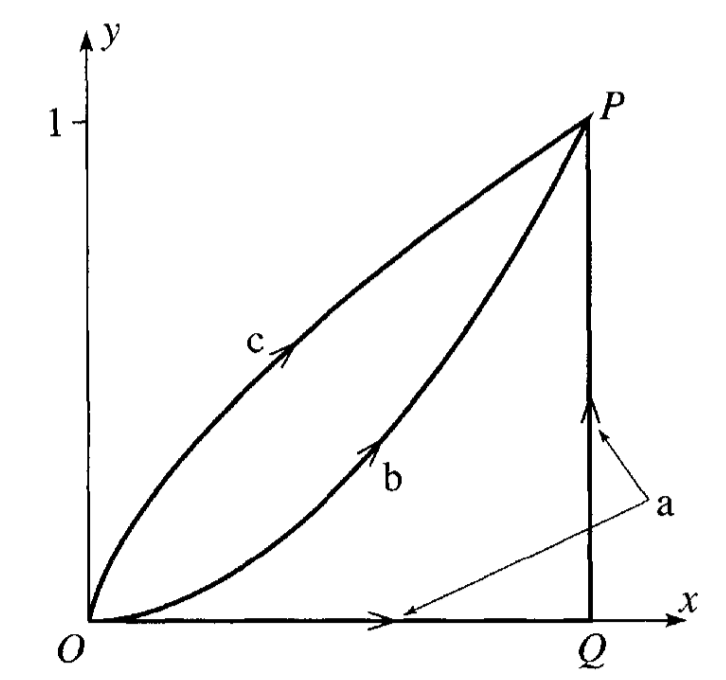
\includegraphics[keepaspectratio,alt={Paths}]{/Users/caballero/repos/teaching/modern-classical-mechanics/content/images/activities/paths.png}}
\caption{Paths}
\end{figure}

In this space, the particle experiences a force:

\[\vec{F} = \langle x^2, 2xy \rangle = x^2\hat{i} + 2xy \hat{j}\]

\begin{itemize}
\tightlist
\item
  1a (3pt) Calculate the work done by the along path \(a\), which is a
  straight line from \((0,0)\) to \((1,0)\), and then to \((1,1)\).
  \emph{Break the path into two segments and calculate the work done
  along each segment separately.}
\item
  1b (3pt) Calculate the work done by the force along path \(b\), which
  follows the function \(y = x^2\) from \((0,0)\) to \((1,1)\).
\item
  1c (4pt) Calculate the work done by the force along path \(c\), which
  is given parametrically by \(x = t^3\) and \(y = t^2\) from \((0,0)\)
  to \((1,1)\).
\item
  1d (5pt) Is this force conservative? Explain your answer in at least
  two ways.
\end{itemize}

    \subsubsection{Exercise 2 (10 pt), Sliding
puck}\label{exercise-2-10-pt-sliding-puck}

A small puck rests on a fixed sphere of radius \(R\). The puck is given
a tiny nudge and it slides down the sphere. Using conservation of
energy, we can determine the point at which the puck leaves the sphere.

\begin{itemize}
\tightlist
\item
  2a (3pt) Setup the problem with a sketch. Explain the setup and
  include any assumptions that you need to make in order to solve the
  problem analytically. Identify the height as a function of the polar
  angle, \(h(\theta)\). What is the maximum possible angle \(\theta\)
  that the puck could reach before falling off? Why?
\item
  2b (2pt) Use conservation of energy to find the speed of the puck as a
  function of it's height. Your answer should be in terms of the polar
  angle, \(\theta\).
\item
  2c (3pt) Use Newton's Second Law to find the normal force acting on
  the puck as a function of it's height. Your answer should be in terms
  of the polar angle, \(\theta\). What is the condition for the puck to
  leave the sphere?
\item
  2d (2pt) At what angle and height does the puck leave the sphere?
\end{itemize}

    \subsubsection{Exercise 3 (10pt), Example of
potential}\label{exercise-3-10pt-example-of-potential}

Consider a particle of mass \(m\) moving according to the potential:

\[
V(x,y,z)=A\exp\left\{-\frac{x^2+z^2}{2a^2}\right\}.
\]

We can think of this potential as the energy landscape of a particle in
three dimensions. That is, you can imagine a particle moving around this
potential like a ball rolling around a landscape. That analogy is not
perfect, but it is a good way to help us think about stability and
equilibrium.

\begin{itemize}
\tightlist
\item
  3a (2pt) Plot this potential or sketch a plot of it. You can use
  perspective plots, contour plots or any other plot you find useful.
\item
  3b (2pt) What are some feature you notice with this potential? What
  happens when you change \(A\) and \(a\)?
\item
  3c (2pt) Imagine a particle moving in this potential, what are some
  expected trajectories?
\item
  3d (2pt) Do there appear to be any equilibrium points? If so, are they
  stable or unstable?
\item
  3a (2pt) Is the resulting force conservative? Why?
\end{itemize}

    \subsubsection{Exercise 4 (15pt), forces and
potentials}\label{exercise-4-15pt-forces-and-potentials}

A particle of mass \(m\) has velocity \(v=\alpha/x\), where \(x\) is its
displacement.

\begin{itemize}
\tightlist
\item
  5a (5pt) Find the force \(F(x)\) responsible for the motion.
\end{itemize}

A particle is thereafter under the influence of a force
\(F=-kx+kx^3/\alpha^2\), where \(k\) and \(\alpha\) are constants and
\(k\) is positive.

\begin{itemize}
\item
  5b (5pt) Determine the potential \(U(x)\) and discuss the motion. It
  can be convenient here to make a sketch/plot of the potential as
  function of \(x\).
\item
  5c (5pt) What happens when the energy of the particle is
  \(E=(1/4)k\alpha^2\)? Hint: what is the maximum value of the potential
  energy?
\end{itemize}

    \subsubsection{Exercise 5 (10pt), Midterms and Final Project
Preparation}\label{exercise-5-10pt-midterms-and-final-project-preparation}

Your final project will be a
\href{https://arxiv.org/abs/1909.12697}{computational essay} of your own
design. My colleague,
\href{https://www.mn.uio.no/fysikk/english/people/aca/toroo/}{Tor Ole
Odden}, and I have borrowed this idea from a proposal by
\href{https://www.stephenwolfram.com/}{Stephen Wolfram}. In his
\href{https://writings.stephenwolfram.com/2017/11/what-is-a-computational-essay}{original
post}, Wolfram talks about the importance of the computational medium as
a way of communicating science.

Tor, myself, and others have started building this idea into a
\href{https://journals.aps.org/prper/abstract/10.1103/PhysRevPhysEducRes.15.020152}{theory
of computational learning in physics}, using computational essays to
\href{https://www-nature-com.proxy2.cl.msu.edu/articles/s41567-023-02371-2}{argue
for the importance of computing in physics}, building
\href{https://pubs-aip-org.proxy2.cl.msu.edu/books/monograph/148/chapter/64396056/Physics-Computational-Literacy-What-Why-and-How}{the
theory out}, and trying to identify the ways making course work and
materials to promote
\href{https://onlinelibrary-wiley-com.proxy2.cl.msu.edu/doi/full/10.1002/tea.21821}{agency,
creativity, and ownership}.

In this homework question, we are going to start building your plan for
your computational essay. I ask that you complete this particular
homework problem by yourself because it is important for each of you to
do this planning.

To get started, you should read the following articles; they are not
very long:

\begin{enumerate}
\def\labelenumi{\arabic{enumi}.}
\tightlist
\item
  Wolfram's
  \href{https://writings.stephenwolfram.com/2017/11/what-is-a-computational-essay}{What
  is a Computational Essay?}
\item
  Tor and my short paper:
  \href{https://arxiv.org/abs/1909.12697}{Computational Essays: An
  Avenue for Scientific Creativity in Physics}
\item
  Wolfram's
  \href{https://www.wolframcloud.com/obj/Expositions/Published/ComputationalEssayGuidelines}{Steps
  to Writing a Computational Essay}
\end{enumerate}

You are, of course, welcome to read more, but these are the three that I
would like you to read.

\begin{itemize}
\tightlist
\item
  5a (3pt) Write a summary of your readings. What did you learn? What
  was important? What did you find interesting? What questions do you
  still have? Full credit will be given for a summary that is at least
  250 words long.
\end{itemize}

Computational essays are a new way to communicate your science. It might
be a good idea to look at some examples. Review the
\href{https://uio-ccse.github.io/computational-essay-showroom}{University
of Oslo's Computational Essay Showroom}.

\begin{itemize}
\tightlist
\item
  5b (3pt) Find at least one computational essay in the
  \href{https://uio-ccse.github.io/computational-essay-showroom}{showroom}
  that you find interesting. Write a summary of the computational essay.
  What did you like? What did you not like? What was interesting about
  it? What questions do you still have? Full credit will be given for a
  summary that is at least 250 words long.
\end{itemize}

These essays were made by students who were taking a course at the
University of Oslo. The essays are not meant to be perfect, they are
meant to be representative of the work that students can do.

\begin{itemize}
\tightlist
\item
  5c (3pt) Evaluate the computational essay based on your readings in
  5a. How well does the computational essay follow the concept of
  physics computational literacy, or the guidelines for a good essay?
  What are the strengths and weaknesses of the computational essay? Full
  credit will be given for a summary that is at least 250 words long.
\end{itemize}

Now, let's move to your future plans.

\begin{itemize}
\tightlist
\item
  5d (1pt) Write a short paragraph about the things you are interested
  in studying for your computational essay. This can be a very short
  paragraph, but it should include at least one image or plot that you
  find interesting. This can be starting from the homework, the samples
  in the showroom, or something else entirely.
\end{itemize}

    \subsubsection{Exercise 6 (40pt), Bouncing
object}\label{exercise-6-40pt-bouncing-object}

This exercise builds on the code you wrote for solving homework 3. We
recommend strongly that you study the text of Malthe-Sørenssen, section
7.5.

In homework 3 we introduced gravity and air resistance and studied their
effects via a constant acceleration due to gravity and the force arising
from air resistance. But what happens when the ball hits the floor? What
if we would like to simulate the normal force from the floor acting on
the ball? This exercise shows how we can include more complicated forces
with no pain! And the force we include here is an example of a case
where analytical solutions may either be difficult to find or we cannot
find an analytical solution at all.

We need then to include a force model for the normal force from the
floor on the ball. The simplest approach to such a system is to
introduce a contact force model represented by a spring model. We model
the interaction between the floor and the ball as a single spring. But
the normal force is zero when there is no contact. Here we define a
simple model that allows us to include such effects in our models.

The normal force from the floor on the ball is represented by a spring
force. This is a strong simplification of the actual deformation process
occurring at the contact between the ball and the floor due to the
deformation of both the ball and the floor.

The deformed region corresponds roughly to the region of
\textbf{overlap} between the ball and the floor. The depth of this
region is \(\Delta y = R-y(t)\), where \(R\) is the radius of the ball.
This is supposed to represent the compression of the spring. Our model
for the normal force acting on the ball is then

    \[
\vec{N} = -k (R-y(t)) \vec{e}_y.
\]

    The normal force must act upward when \(y < R\), hence the sign must be
negative. However, we must also ensure that the normal force only acts
when the ball is in contact with the floor, otherwise the normal force
is zero. The full formation of the normal force is therefore

    \[
\vec{N} = -k (R-y(t)) \vec{e}_y,
\]

    when \(y(t) < R\) and zero when \(y(t) \ge R\). In the numerical
calculations you can choose \(R=0.1\) m and the spring constant
\(k=1000\) N/m.

\begin{itemize}
\item
  6a (10pt) Identify the forces acting on the ball and set up a diagram
  with the forces acting on the ball. Find the acceleration of the
  falling ball now with the normal force as well.
\item
  6b (30pt) Choose a large enough final time so you can study the ball
  bouncing up and down several times. Add the normal force and compute
  the height of the ball as function of time with and without air
  resistance. Comment your results.
\end{itemize}

    \subsubsection{Integrating Classwork With
Research}\label{integrating-classwork-with-research}

This opportunity will allow you to earn up to 5 extra credit points on a
Homework per week. These points can push you above 100\% or help make up
for missed exercises. In order to earn all points you must:

\begin{enumerate}
\def\labelenumi{\arabic{enumi}.}
\item
  Attend an MSU research talk (recommended research oriented Clubs is
  provided below)
\item
  Summarize the talk using at least 150 words
\item
  Turn in the summary along with your Homework.
\end{enumerate}

Approved talks: Talks given by researchers through the following clubs:

\begin{itemize}
\item
  Society for Physics Students (SPS)\hspace{0pt}: Meets Monday Nights
  (alternates with Astronomy Club)
\item
  Astronomy Club\hspace{0pt}: Meets Monday Nights (alternates with SPS)
\item
  Any \href{https://pa.msu.edu/news-events-seminars/index.aspx}{physics
  and astronomy seminar} of interest to you
\end{itemize}

If you have any questions please consult Danny.

    


    % Add a bibliography block to the postdoc
    
    
    
\end{document}
